% !TEX root = ../main.tex
% !TEX program = xelatex
\section{问题一的模型建立与求解}

%====================
\subsection{求解思路与模型选择}

问题一已知一天内各时段的负载、光伏预测和电价，需要确定外网购电量以及储能设备的充放电安排，在满足负载需求和储能运行约束的前提下，使全天购电费用尽可能低。
同时，题目要求0:00与24:00的储电量相同。

由前文探索性分析可知，午间容易出现光伏富余，而较大的供需缺口和较高电价更多出现在傍晚。
因此，当前时段是否充放电，会直接影响后续可使用的储能。若仅采用“低价充电、高价放电”的简单规则，可能过早充满或放空电池，错过后续更有价值的调节时机。

基于这一特点，本文首先考虑两种较直观的调度思路作为对照。
第一种为\textbf{峰谷电价策略}，按照“低价充电、高价放电”的原则，根据电价门槛安排储能；
第二种为\textbf{光伏空间预留策略}，在峰谷电价策略基础上，结合午间光伏富余的特点，为后续光伏预留一定储能空间。

这两种规则策略能够反映较直观的调度思路，但都需要事先设定价格门槛或目标储电量，难以同时考虑当前充放电行为对后续高价时段和光伏富余时段的影响。
为此，本文进一步将全天144个10分钟时段统一考虑，同时优化各时段的购电、充电和放电安排。

由于购电费用、供需平衡、储电量变化以及容量和充放电功率约束均可表示为线性关系，因此建立\textbf{线性规划模型}。
后续在相同的代表日数据、充放电效率和首尾储电量条件下，将线性规划与上述两种规则策略进行比较，并根据实际购电费用确定最终采用的方案。

%====================
\subsection{问题一的模型建立}

\subsubsection*{（1）时段与电量划分}

将一天划分为144个10分钟时段，记为
\[
k=1,2,\ldots,144,\qquad \Delta t=\frac{1}{6}\text{ h}.
\]

第 \(k\) 个时段的负载电量和光伏电量分别为
\begin{equation}
E_k^L=L_k\Delta t,\qquad
E_k^{PV}=P_k^{PV}\Delta t.
\label{eq:q1_energy}
\end{equation}

按照“光伏优先满足负载”的原则，定义光伏直接供给负载的电量为
\[
m_k=\min(E_k^L,E_k^{PV}),
\]
进一步得到光伏直供后的负载缺口和光伏富余量：
\begin{equation}
n_k=E_k^L-m_k,\qquad
r_k=E_k^{PV}-m_k.
\label{eq:q1_gap_surplus}
\end{equation}

其中，\(n_k\) 表示该时段仍需由外网或储能补充的电量，\(r_k\) 表示可用于储能的富余光伏。

\subsubsection*{（2）决策变量与电量流向}

设
\[
x_k:\text{外网用于储能充电的电量},
\]
\[
y_k:\text{富余光伏用于储能充电的电量},
\]
\[
z_k:\text{储能向负载放出的电量},
\]
\[
S_k:\text{第 }k\text{ 时段结束时的储电量}.
\]

各类电量之间的关系如图~\ref{fig:q1_1}所示。光伏优先直接满足负载，富余部分可用于储能；外部电网既可直接补足负载，也可为储能充电；储能则在需要时向负载放电。

\begin{figure}[H]
    \centering
    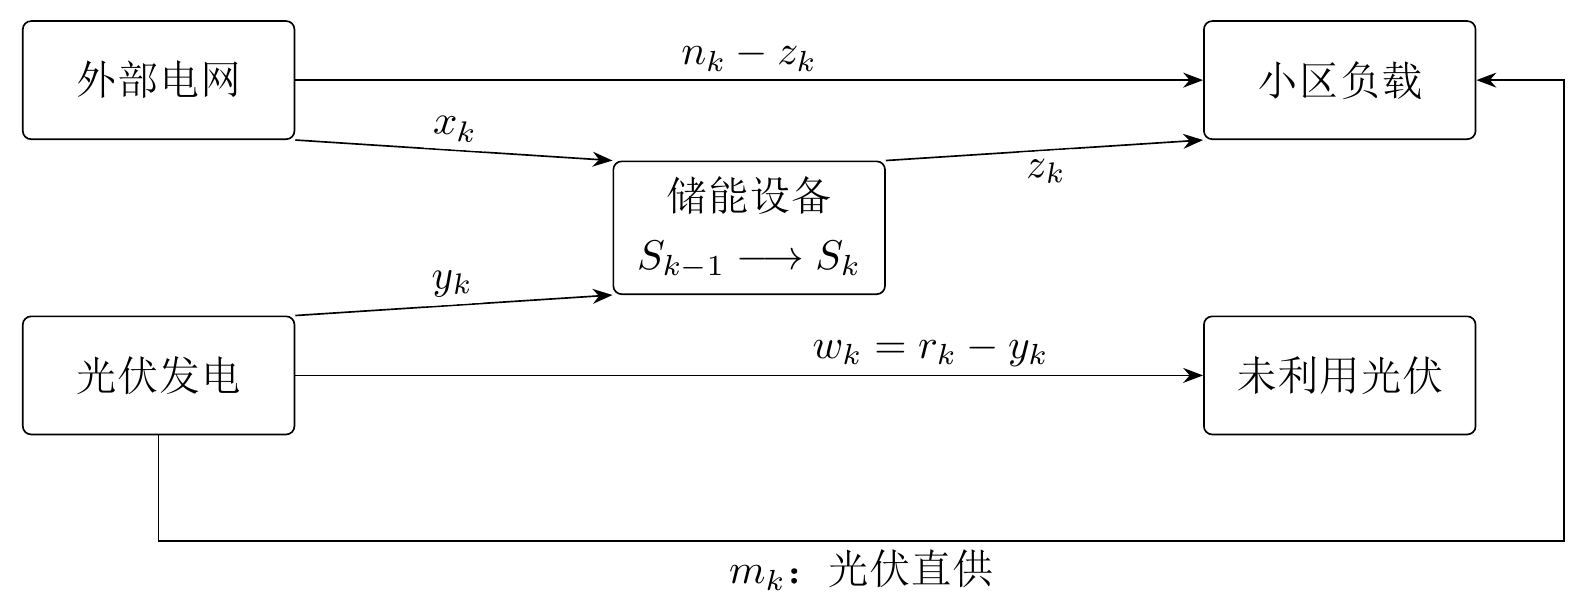
\includegraphics[width=0.95\textwidth]{fig/q1_1.png}
    \caption{问题一的电量分配关系}
    \label{fig:q1_1}
\end{figure}

因此，第 \(k\) 个时段的外网购电量为
\begin{equation}
q_k=n_k-z_k+x_k.
\label{eq:q1_purchase}
\end{equation}

未被利用的光伏量为
\[
w_k=r_k-y_k.
\]

\subsubsection*{（3）目标函数}

问题一只计算外网购电费用，因此以全天购电费用最小为目标：
\begin{equation}
\min C=
\sum_{k=1}^{144}
p_k\left(n_k-z_k+x_k\right),
\label{eq:q1_objective}
\end{equation}
其中，\(p_k\) 为第 \(k\) 个时段的电价。

该目标最小化的是\textbf{购电费用，而不是购电总量}。因此，模型允许在低价时段适当多购电，并通过储能减少后续高价时段的购电。

\subsubsection*{（4）约束条件}

为保证购电与储能调度方案能够实际执行，模型需同时满足供需平衡、充放电功率、储电容量以及日首尾储电量约束。

\textbf{1）供需与光伏利用约束}

光伏直供后，剩余负载由外网和储能共同补足；富余光伏可用于储能，但不能超过该时段实际可用的光伏余量。因此有
\begin{equation}
x_k\geq 0,\qquad
0\leq y_k\leq r_k,\qquad
0\leq z_k\leq n_k.
\label{eq:q1_supply_constraint}
\end{equation}

其中，\(y_k\leq r_k\) 保证光伏充电量不超过富余光伏，\(z_k\leq n_k\) 保证储能放电量不超过当前负载缺口。结合前文
\[
q_k=n_k-z_k+x_k,
\]
可保证每个时段的负载均得到满足。

\textbf{2）储能充放电功率约束}

储能设备最大充电功率和放电功率均为 \(5000\,\mathrm{kW}\)。每个调度时段为10分钟，因此单个时段的充电量和放电量均不能超过 \(833.33\,\mathrm{kWh}\)：

\begin{equation}
x_k+y_k\leq833.33,\qquad
z_k\leq833.33.
\label{eq:q1_power_constraint}
\end{equation}

该约束限制的是储能设备的充放电能力，不限制外网直接向小区负载供电。

\textbf{3）储电量变化与容量约束}

储能设备的充电效率和放电效率均为 \(90\%\)。因此，第 \(k\) 个时段结束后的储电量满足

\begin{equation}
S_k
=
S_{k-1}
+0.9(x_k+y_k)
-\frac{z_k}{0.9}.
\label{eq:q1_soc_transition}
\end{equation}

同时，为避免过度充电或放电，储电量始终保持在允许范围内：

\begin{equation}
1200\leq S_k\leq10800,
\qquad k=1,2,\ldots,144.
\label{eq:q1_soc_bound}
\end{equation}

式~\eqref{eq:q1_soc_transition}同时考虑了充电和放电过程中的能量损耗。

\textbf{4）日首尾储电量约束}

问题一要求0:00和24:00的储电量相同。主方案初始储电量取 \(6000\,\mathrm{kWh}\)，因此有

\begin{equation}
S_0=S_{144}=6000\ \mathrm{kWh}.
\label{eq:q1_terminal_constraint}
\end{equation}

该约束避免模型通过消耗原有储电量来降低当天表面购电费用，使不同调度方案在相同的起点和终点下进行比较。

%====================
\subsection{问题一的模型求解}

上述目标函数和约束均为线性关系，因此可直接采用线性规划求解。模型每个时段包含 \(x_k\)、\(y_k\)、\(z_k\) 和 \(S_k\) 四个连续变量，全天共576个连续变量，各时段通过储电量递推关系相互连接。

在本题电价为正、外网能够直接供给负载的条件下，同一时段同时充电和放电只会增加储能损耗，因此无需额外设置0--1变量限制充放电状态。

本文采用 Python 中 SciPy 的 \texttt{linprog} 接口调用 HiGHS 求解器。主要计算步骤如下：

\begin{enumerate}
    \item 将负载和光伏功率转换为各10分钟时段的电量；
    \item 根据式~\eqref{eq:q1_gap_surplus}计算各时段的负载缺口和光伏富余量；
    \item 建立目标函数及储能运行约束；
    \item 求解各时段的购电量、充放电量和储电量。
\end{enumerate}

为判断线性规划的实际效果，本文同时设置两种规则策略作为对照：

\begin{itemize}
    \item \textbf{峰谷电价策略：}低价时充电，高价时放电；
    \item \textbf{光伏空间预留策略：}在峰谷策略基础上，为后续富余光伏预留储能空间。
\end{itemize}

两种规则均考察27组参数组合，其中低价门槛分别取电价的15\%、25\%、35\%分位，高价门槛取65\%、75\%、85\%分位，目标储电量取6000、8400和10800 kWh，并分别选择已考察组合中费用最低的方案与线性规划比较。

%====================
\subsection{求解结果与分析}

\subsubsection*{（1）最终购电方案}

线性规划得到全天购电量为
\[
\boxed{59482.70\ \mathrm{kWh}},
\]
全天购电费用为
\[
\boxed{35126.85\ \mathrm{元}}.
\]

储能设备全天累计充电量为 \(20740.67\,\mathrm{kWh}\)，累计放电量为 \(16799.94\,\mathrm{kWh}\)。

题目要求的重点时段购电结果如表~\ref{tab:q1_purchase_result}所示。

\begin{table}[H]
    \centering
    \caption{微网在指定时间段的购电量及全天的购电量和购电费 }
    \label{tab:q1_purchase_result}
    \begin{tabular}{|c|c|c|c|c|c|}
        \hline
        时间段 & 购电量 & 时间段 & 购电量 & 时间段 & 购电量 \\
        \hline
        10:00-10:10 & \textbf{0.00} & 12:00-12:10 & \textbf{486.40} & 14:00-14:10 & \textbf{0.00} \\
        \hline
        16:00-16:10 & \textbf{394.93} & 18:00-18:10 & \textbf{636.98} & 20:00-20:10 & \textbf{0.00} \\
        \hline
        \multicolumn{2}{|c|}{全天购电量} & \multicolumn{1}{c|}{\textbf{59482.70}} & \multicolumn{2}{c|}{全天购电费} & \multicolumn{1}{c|}{\textbf{35126.85}}\\
        \hline
    \end{tabular}
\end{table}

储能设备各4小时区间的充放电结果如表~\ref{tab:q1_storage_result}所示。

\begin{table}[H]
    \centering
    \caption{问题一各4小时区间的储能充放电量}
    \label{tab:q1_storage_result}
    \begin{tabular}{|c|c|c|c|c|c|}
        \hline
        时间段 & 充电量 & 放电量 & 时间段 & 充电量 & 放电量 \\
        \hline
        00:00--04:00 & \textbf{4500.00} & \textbf{0.00} & 04:00--08:00 & \textbf{833.33} & \textbf{5947.42} \\
        \hline
        08:00--12:00 & \textbf{3954.63} & \textbf{2121.42} & 12:00--16:00 & \textbf{6119.37} & \textbf{91.10} \\
        \hline
        16:00--20:00 & \textbf{0.00} & \textbf{5068.69} & 20:00--24:00 & \textbf{5333.33} & \textbf{3571.31} \\
        \hline
        \multicolumn{2}{|c|}{0:00储电量} & \multicolumn{1}{|c|}{\textbf{6000.00}} & \multicolumn{2}{c|}{24:00储电量} & \multicolumn{1}{c|}{\textbf{6000.00}}\\
        \hline
    \end{tabular}
\end{table}

某个4小时区间内同时出现充电量和放电量，只表示这些行为发生在不同的10分钟时段，并不表示同一时段同时充放电。

\subsubsection*{（2）三种策略比较}

针对5.1中提出的三种策略：峰谷电价策略、光伏空间预留策略和线性规划，我们分别计算了它们对应的全天购电费用，如表~\ref{tab:q1_strategy_compare}所示。

\begin{table}[H]
    \centering
    \caption{三种策略的全天购电费用比较}
    \label{tab:q1_strategy_compare}
    \begin{tabular}{cc}
        \toprule
        策略 & 全天购电费/元 \\
        \midrule
        峰谷电价策略 & 38276.64 \\
        光伏空间预留策略 & 37944.35 \\
        线性规划 & \textbf{35126.85} \\
        \bottomrule
    \end{tabular}
\end{table}

线性规划相比峰谷电价策略节省 \(3149.79\) 元，降幅为 \(8.23\%\)；相比光伏空间预留策略节省 \(2817.50\) 元，降幅为 \(7.43\%\)。

这也证实了我们\textbf{选择线性规划作为问题一的最终调度模型}的正确性。

\subsubsection*{（3）节费原因分析}

三种策略全天的电价、储电量和外网购电变化如图~\ref{fig:q1_2}所示。

\begin{figure}[H]
    \centering
    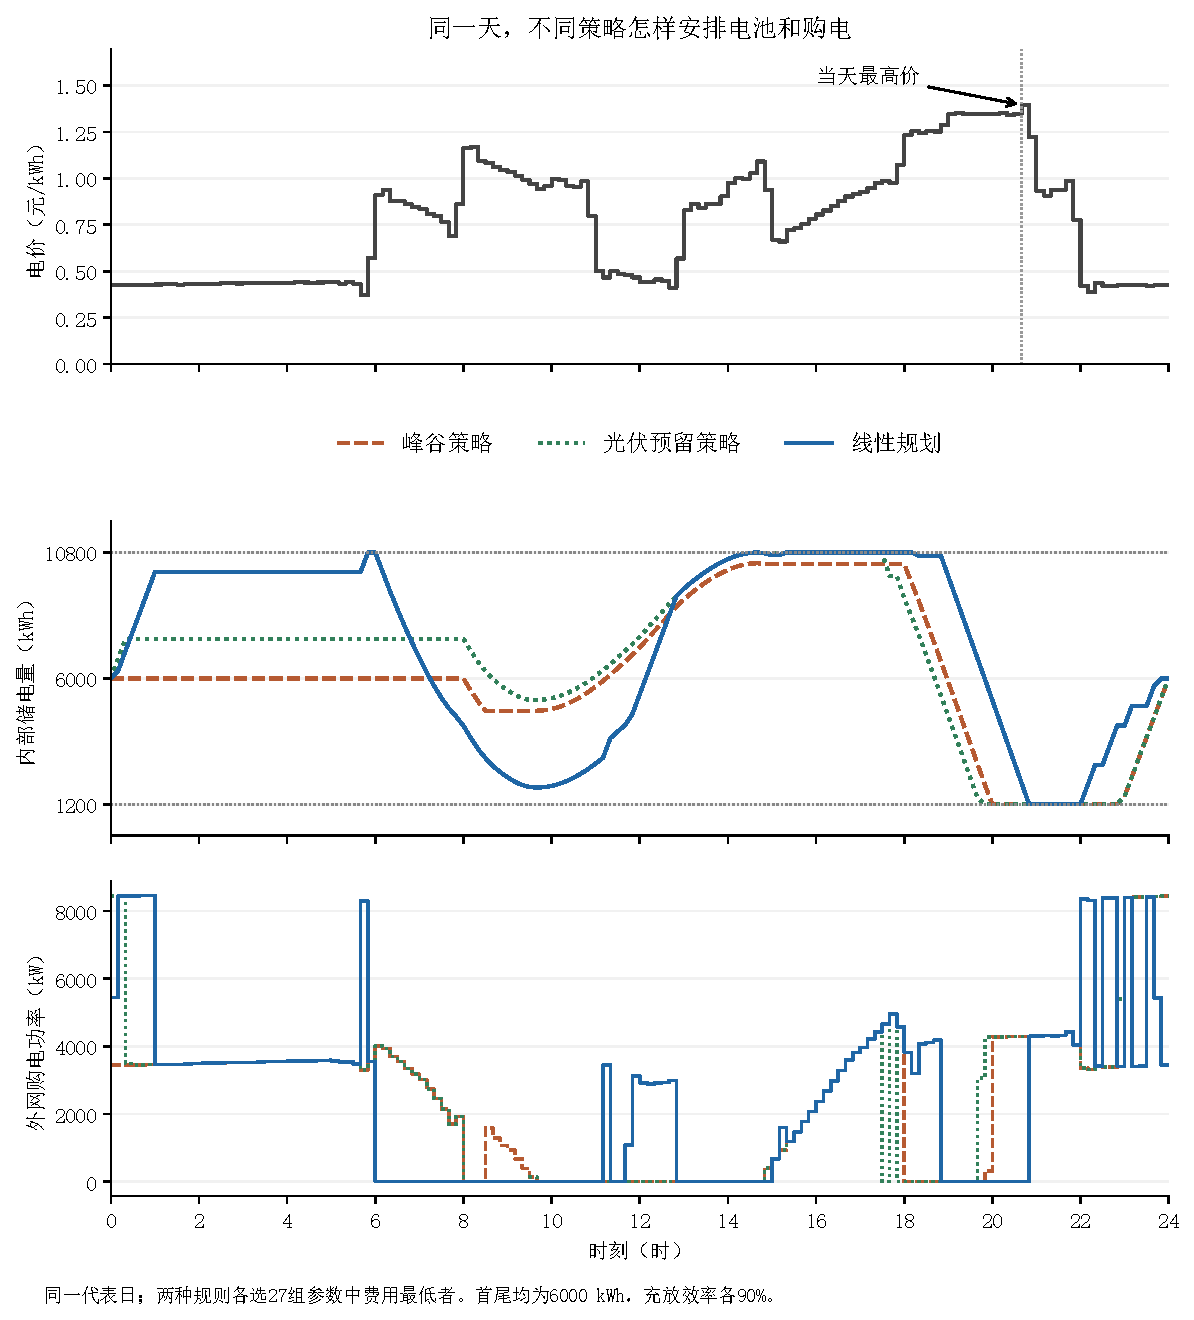
\includegraphics[width=0.95\textwidth]{fig/q1_daily_dispatch.pdf}
    \caption{三种策略在相同代表日下的购电与储能安排}
    \label{fig:q1_2}
\end{figure}

从图~\ref{fig:q1_2}可以看出，线性规划并不是一进入高价时段就立即放空电池，而是会将部分电量保留给后续更高价格的时段。

20:00时，两种规则策略的储电量已经降至 \(1200\,\mathrm{kWh}\) 下限，而线性规划仍保留 \(5168.13\,\mathrm{kWh}\)。
当20:40--20:50的电价达到全天最高的 \(1.3952\,\mathrm{元/kWh}\) 时，线性规划利用储能满足负载，该时段外网购电量为0；另外两种策略则需要购买 \(715.65\,\mathrm{kWh}\) 的高价电。

因此，线性规划节费的关键并不是简单的“低价充、高价放”，而是根据全天价格变化，\textbf{将有限的储能优先留给更有价值的高价时段}。

值得注意的是，线性规划相比峰谷策略多购电 \(1740.28\,\mathrm{kWh}\)。这是因为更多电量经过储能后会产生损耗。但增加的购电主要发生在低价时段，并替代了后续更加昂贵的购电，因此最终总费用仍然更低。

%====================
\subsection{模型检验与敏感性分析}

\subsubsection*{（1）模型结果检验}

为保证求解结果可信，本文重新计算各10分钟时段的供需平衡、储电递推、容量限制、充放电功率和全天费用，并核对日初与日末储电量。

三个初始储电案例中的最大储电递推残差约为
\[
1.34\times10^{-12}\ \mathrm{kWh},
\]
求解费用与对应下界的最大差值约为
\[
1.22\times10^{-12}\ \mathrm{元}.
\]

二者均处于数值计算误差范围内，说明所得结果满足模型约束，并支持当前线性规划解的数值最优性。

\subsubsection*{（2）初始储电量敏感性分析}

为考察初始储电量对结果的影响，在其他条件保持不变的情况下，分别取
\[
S_0=1200,\qquad 6000,\qquad 10800\ \mathrm{kWh},
\]
并在每种情况下重新优化，同时要求24:00恢复到相同的初始储电量。

结果如表~\ref{tab:q1_sensitivity}所示。

\begin{table}[H]
    \centering
    \caption{不同初始储电量下的购电费用}
    \label{tab:q1_sensitivity}
    \begin{tabular}{ccc}
        \toprule
        初始储电量/kWh & 全天购电费用/元 & 相比6000 kWh方案 \\
        \midrule
        1200 & 35199.30 & $+0.21\%$ \\
        6000 & \textbf{35126.85} & --- \\
        10800 & 35409.75 & $+0.81\%$ \\
        \bottomrule
    \end{tabular}
\end{table}

三个方案与主方案的费用差异均不足 \(1\%\)，且都会为晚间最高价时段保留电量。这说明初始储电量会改变部分具体购电时刻，但不会改变“将有限储能留给更高价值时段”这一主要调度规律。

需要说明的是，该敏感性分析仅检验了上述三个初始储电量，因此不能据此认定 \(6000\,\mathrm{kWh}\) 是整个允许区间内的最优初始状态。